\section{Bidirectional search \cite{ai/book/Artificial-Intelligence-A-Modern-Approach/Russell-Norvig}}
\label{AI: Algorithms/Bidirectional search}

\begin{figure}[h!]
    \centering
    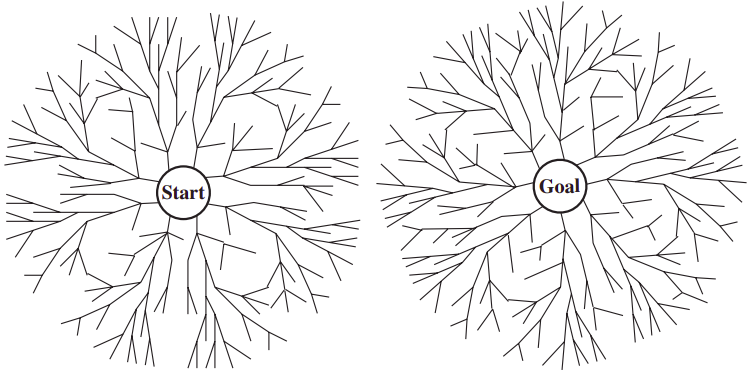
\includegraphics[
        width=\linewidth,
        height=4cm,
        keepaspectratio,
    ]{images/algorithms/bidirectional-search-illustration.png}
    \caption*{A schematic view of a bidirectional search that is about to succeed when a branch from the start node meets a branch from the goal node. \cite{ai/book/Artificial-Intelligence-A-Modern-Approach/Russell-Norvig}}
\end{figure}


\begin{enumerate}
    \item The idea behind bidirectional search is to run two simultaneous searches - one forward from the initial state and the other backward from the goal - hoping that the two searches meet in the middle
    \hfill \cite{ai/book/Artificial-Intelligence-A-Modern-Approach/Russell-Norvig}

    \item The motivation is that $b^{d/2} + b^{d/2}$ is much less than $b^d$
    \hfill \cite{ai/book/Artificial-Intelligence-A-Modern-Approach/Russell-Norvig}

    \item Bidirectional search is implemented by replacing the goal test with a check to see whether the frontiers of the two searches intersect; if they do, a solution has been found.
    \hfill \cite{ai/book/Artificial-Intelligence-A-Modern-Approach/Russell-Norvig}

    \item The check can be done when each node is generated or selected for expansion and, with a hash table, will take constant time.
    \hfill \cite{ai/book/Artificial-Intelligence-A-Modern-Approach/Russell-Norvig}

    \item \textbf{predecessors} of a state $x$ be all those states that have $x$ as a successor. Bidirectional search requires a method for computing predecessors. When all the actions in the state space are reversible, the predecessors of $x$ are just its successors. 
    \hfill \cite{ai/book/Artificial-Intelligence-A-Modern-Approach/Russell-Norvig}

    \item \textbf{Performance}:
    \begin{enumerate}
        \item \textbf{optimality}: 
        \begin{enumerate}
            \item YES \textbf{if} additional search is used to make sure the path isn’t another short-cut across the gap \textbf{else} NO
            \hfill \cite{ai/book/Artificial-Intelligence-A-Modern-Approach/Russell-Norvig}

            \item YES \textbf{if}  step costs are all identical \textbfit{and} both directions use breadth-first search \textbf{else} NO
            \hfill \cite{ai/book/Artificial-Intelligence-A-Modern-Approach/Russell-Norvig}
        \end{enumerate}

        \item \textbf{completeness}: YES \textbf{if} $b$ is finite \textbfit{and} both directions use breadth-first search \textbf{else} NO
        \hfill \cite{ai/book/Artificial-Intelligence-A-Modern-Approach/Russell-Norvig}

        \item \textbf{space complexity}:
        \begin{enumerate}
            \item using breadth-first searches in both directions: $\mathcal{O}(b^{d/2})$
            \hfill \cite{ai/book/Artificial-Intelligence-A-Modern-Approach/Russell-Norvig}
        \end{enumerate}

        \item \textbf{time complexity}:
        \begin{enumerate}
            \item using breadth-first searches in both directions: $\mathcal{O}(b^{d/2})$
            \hfill \cite{ai/book/Artificial-Intelligence-A-Modern-Approach/Russell-Norvig}
        \end{enumerate}
    \end{enumerate}
\end{enumerate}






















